\lab{Algorithms}{The Natural Embedding Algorithm}{Bifurcations}
\label{lab:Bifurcations}

The flow of a differential equation \[\dot{x} = f(x)\] is the family of all possible solutions $\phi(t,x_0)$, where $x_0$ represents the arbitrary initial value, $t \in \mathbb{R}.$ Here we will mainly consider scalar differential equations (so-called because $x$ is one dimensional). It is often necessary to study a family of differential equations. These will have the form 
\[\dot{x}= F(x,c),\]
where $c$ may be a single parameter or a vector of parameters. 

Bifurcation theory is the study of how the qualitative structure of the flow of a differential equation varies as parameters in the differential equation are varied. 
A differential equation has a stable orbit structure if sufficiently small changes in the parameter value do not change the qualitative structure of the flow.
A parameter value for which the flow does not have a stable orbit structure is called a bifurcation value.
A bifurcation diagram is ...

% Terminology
% bifurcation theory: 'the study of possible changes in the structure of orbits of a differential equation depending on variable parameters'
% 'the study of changes in the qualitative structure of the flow of a differential equation as parameters are varied'
% phase portrait: 
% bifurcation diagram: 
% number of orbits and their direction of flow of a differential equation = 'orbit structure of the differential equation' or 'the qualitiative structure of the flow'.
%  

% Hyperbolic equilibrium points
% $F(x_0,c_0) = 0$ where $\frac{df}{dx}(x_0,c_0) \not = 0.$ In this case the stability of the equilibrium point $x_0$ for values of $c$ near $c_0$ is determined by the derivative $\frac{df}{dx}(x_0,c_0)$.
% Example: $\dot{x} = x-c.$ Plot $x$


% Hyperbolic equilibrium - mainly to be used when discussing stability
% Saddle-Node Bifurcation - \[\dot{x} = c + x^2.\]
% Transcritical Bifurcation - \[\dot{x} = cx + x^2.\]
% Hysteresis Loop - \[\dot{x} = c + x-x^3.\]
% Pitchfork Bifurcation (Supercritical) - \[\dot{x} = cx-x^3.\]
% For an exercise, do a variation of \[\dot{x} = 1+cx-x^3.\]
% 
% For examples, use first three
Consider the scalar differential equation 
\begin{eqnarray}
\dot{x} &=& c + x^2. \label{snbifurcation}
\end{eqnarray}
For $c>0$ equation (\ref{snbifurcation}) has no equilibrium solutions. At $c=0$ the equilibrium point $x=0$ appears, and for $c<0$ it splits into two equilibrium points. For this system, a bifurcation occurs at $c=0$. This is an example of a saddle-node bifurcation. The bifurcation diagram is shown in Figure \ref{bifurcation:sn} 


\begin{figure}[ht]
\centering
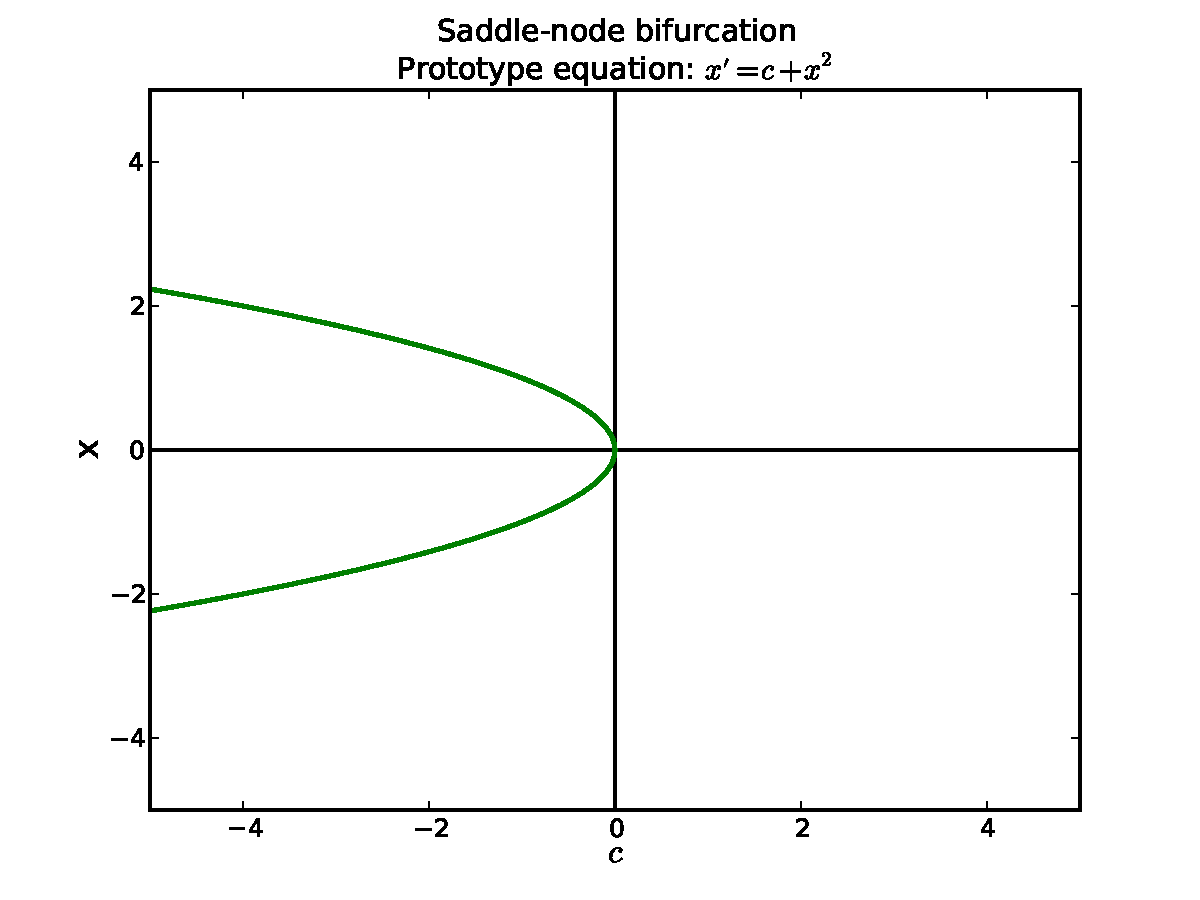
\includegraphics[width=\textwidth]{SaddleNBifurcation.pdf}
\caption{Bifurcation diagram for the equation $\dot{x} = c + x^2$.}
\label{bifurcation:sn}
\end{figure}

Here we describe a method for solving for these equilibrium points called the natural embedding algorithm. This version of the natural embedding algorithm uses Newton's method to solve for the zeros of $F(x,c).$ Once a solution $x_0$ is known for a parameter value $c_0$, that value $x_0$ can be used as an initial guess for the solution $x_1$ corresponding to the next parameter value $c_1$.

The following code implements the natural embedding algorithm, and then uses that algorithm to create the bifurcation diagram in Figure \ref{bifurcation:sn}

\begin{lstlisting}
import numpy as np
import matplotlib.pyplot as plt
from scipy.optimize import newton

def EmbeddingAlg(c_list,Initial_Guess,F):
	X = []
	for c in c_list:
		try:
			g = lambda x,c = c: F(x,c)
			Solution = newton(g, Initial_Guess, fprime=None, args=(), tol=1.0e-08, maxiter=50)
			Initial_Guess = Solution # Intial Guess updated for the next iteration
			X.append(Solution)
		except:
			return c_list[:len(X)], X	
	return c_list[:len(X)], X   		
	# returns the list of c values that it was able to find  
	# corresponding values of x for, along with those 					
	# x values
	
	
def SaddleNode_bifurcation():
	def F(x,c):
		return c + x**2
	
	T = np.linspace(0,5,500)
	plt.plot(T,np.zeros(T.shape),'-k')   # Graph x and c axes
	plt.plot(-T,np.zeros(T.shape),'-k')
	plt.plot(np.zeros(T.shape),T,'-k')
	plt.plot(np.zeros(T.shape),-T,'-k')
	
	C,X = EmbeddingAlg(np.linspace(-5,0,500),np.sqrt(5),F)
	plt.plot(C,X,'-g',linewidth=2.0)
	C,X = EmbeddingAlg(np.linspace(-5,0,500),-np.sqrt(5),F)
	plt.plot(C,X,'-g',linewidth=2.0)
	
	plt.axis([-5,5,-5,5])
	plt.title("Saddle-node bifurcation\n Prototype equation: $x' = c + x^2$")
	plt.xlabel('$c$',fontsize=16)
	plt.ylabel('x',fontsize=16)
	plt.show()
	return

SaddleNode_bifurcation()

\end{lstlisting}
% 
% Let us look at the equilibrium points of a specific example, 
% \[\dot{x}= x^2 +c.\]
% For $c>0,$ there are no fixed points for this system. The vector field described by $F(x,c)$ moves every point to $+\infty$ as $t \to\infty$. 

% \section*{Insert Section Name Here}
% 
\begin{problem}
Use the natural embedding algorithm to create a bifurcation diagram for the differential equation
\[\dot{x} = cx-x^3.\]
This type of bifurcation is called a pitchfork bifurcation (look for a pitchfork in your diagram).
\end{problem}

\begin{problem}
Use the natural embedding algorithm to create a bifurcation diagram for the differential equation
	\[\dot{x} = c + x - x^3.\]
You should see two saddle-node bifurcations in your diagram. 
\end{problem}

\begin{problem}
Create bifurcation diagrams for the differential equation
\[\dot{x} = d + cx-x^3,\]
where $d = -1., -.2, .2$ and $1.$

\end{problem}



%\li{ode} 
%
%\begin{lstlisting}
%
%\end{lstlisting}